\documentclass{article}

\usepackage{amsmath}
\usepackage{tikz}
\usepackage{url}
\usepackage[linesnumbered,ruled]{algorithm2e}
\usepackage[toc,page]{appendix}
\usetikzlibrary{backgrounds,positioning}
\usetikzlibrary{decorations.pathreplacing}

\tikzset{
  cell/.style = {rectangle, draw, text width=1.3cm, outer sep=0pt},
  capx/.style = {rectangle, draw, text width=1.3cm, color=black!40,outer sep=0pt}
}

\title{Efficient Implementation of the TKF91-Model}

\author{Pierre Barbera and Sarah Lutteropp}

\begin{document}
\maketitle

\begin{abstract}
In this document we explain the optimizations we undertook in order to produce an efficient implementation of the TKF91 model by Thorne, Kishino and Felsenstein. We transformed the algorithm into log-space to avoid numerical underflow. This also allowed us to further simplify the formulas. Moreover, we improved data locality by storing the matrix entries in a special data structure. While we also tried different vectorization techniques, it turned out that our fastest code used no vectorization at all. We conclude that we simplified the sequential code to an extent that the benefit of using SIMD instructions cannot compensate for the additional overhead we need for vectorization.
\end{abstract}

\section{Mathematical Optimization}

\paragraph{Numerical Underflow Prevention}
\label{sec:log}

As the TKF91 algorithm~\cite{Thorne91tkf} performs successive multiplications on, in practice,
limited precision floating point numbers, numerical underflow presented a major
challenge. This already became an issue for short input sequences, well below $100$ nucleotides.
To resolve this issue we decided to transform all computations into log-space, adding up logarithms of probabilities instead of multiplying them.
While it is still possible to experience under- or overflow after this transformation, it is highly unlikely for practical inputs.
Consequently we did not observe any numerical underflow for the tested input parameters and sequence lengths up to and including $10000$ nucleotides.

\paragraph{Simplifying the Formulas}  
We were able to get rid of redundant computations be reusing the already computed values for previous matrix entries.
For example, we observed that $$M^0(i+1,0) = M^0(i,0) + \log(\gamma_{i+1}) + \log(\zeta_{i+1}) + \log(\beta(t)) + \log(\pi_{a_{i+1}}) + \log(\bar{p_0}(t)).$$
After replacing $\beta(t), \bar{p_0}(t), \gamma_i$ and $\zeta_i$ by their formulas in the computation of the matrix entries, we observed that some terms reappeared multiple times. 
Operating in log-space allowed us to further simplify the formulas. Especially the logarithmic rules $\log(a*b) = \log(a) + \log(b)$ and $\log(a/b) = \log(a) - \log(b)$ allowed us to replace multiplications and divisions with additions and subtractions.
The resulting formulas can be found in Appendix~\ref{sec:formulas}.

\paragraph{Precomputing the Logarithms}
While replacing a multiplication with two logarithm operations is more costly in general, we did not experience any computational overhead. This is because our formulas consist of sums of only $25$ different logarithms which we precomputed in the code.

A major downside of using logarithmic transformation is that any error in its original computation accumulates over the runtime of the program. This occurs because we add up the logarithms multiple times. To investigate this further, we used the high precision mathematical library of the \texttt{boost}-framework \cite{boost}. It utilizes data types that can dynamically extend their floating point precision to avoid numerical errors and under/overflow. Our basic idea was to use this library only during precomputation, limiting its added overhead. However transforming these data types back into standard double values proved to be problematic, as it introduced additional loss of precision. As a consequence we decided to abandon this path.

\section{Matrix Storage}
\label{sec:caching}

\paragraph{Matrix as Array}
In the naive approach, we stored each of the matrices $M^0, M^1$ and $M^2$ in a separate array, using row-major order. The matrix index at position $(i,j)$ corresponds to the index position $i*(m+1)+j$ in its array (see Figure~\ref{fig:rowmajor}).

To visualize the shortcomings of this approach, we can use the following example: we assume that six rows of one matrix fit into one cache line. Performing one iteration of the main computation loop then has to load three cache lines: one per matrix. This is depicted in part a) of Figure~\ref{fig:cachelines}.
If we further assume that only two cache lines fit into the cache at one time, every iteration would then cause one of the lines to be swapped out, causing memory overhead.

\begin{figure}
\centering
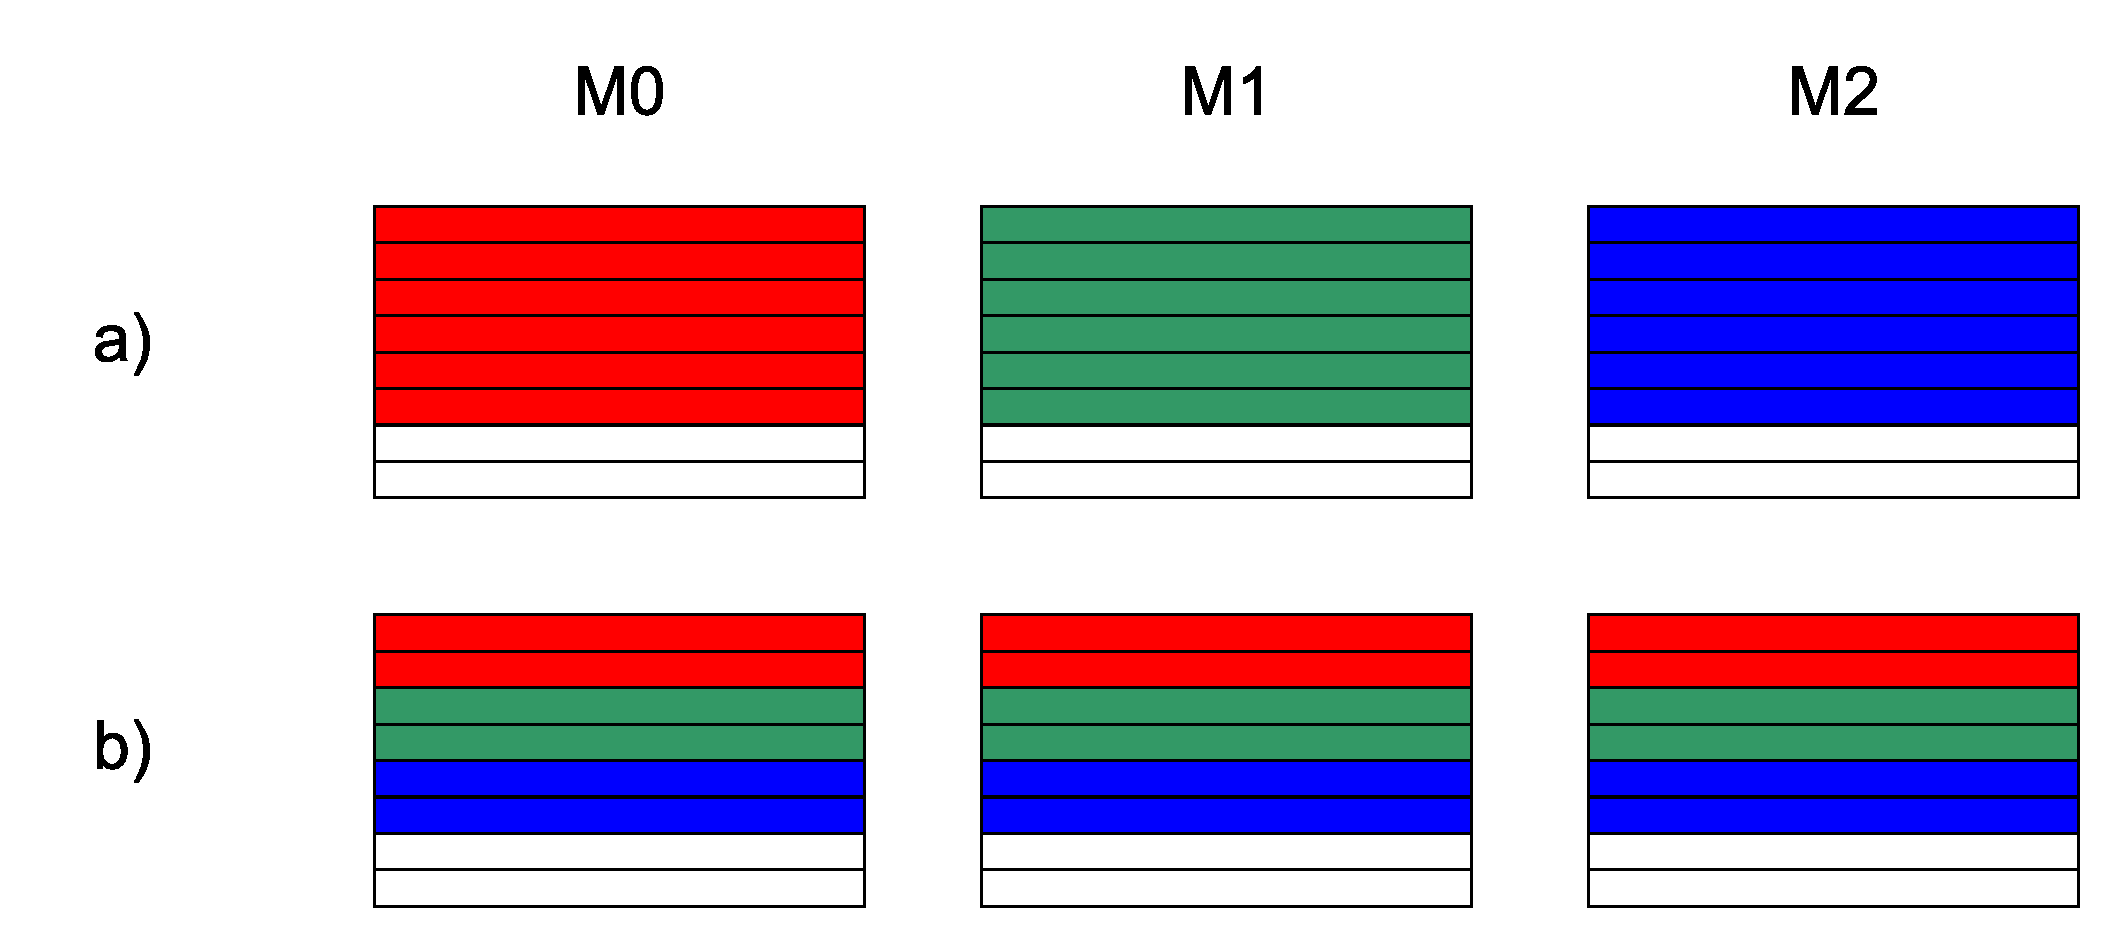
\includegraphics[width=\textwidth]{images/cachelines.pdf}
\caption{Relation of cache lines and matricies, using the method of allocating each matrix separately(\textbf{a)}) and the Array-of-Structs method (\textbf{b)}). Each color signifies a different cache line.}
\label{fig:cachelines}
\end{figure}

\paragraph{Array-of-Structs Data Structure}
The dynamic programming step (see Algorithm~\ref{alg:dp}) accesses the matrices $M^0, M^1$ and $M^2$ by the same index position in order to find the maximum entry. Thus we decided to improve data locality by storing the entries from matrices found at the same index position next to each other in memory. For this, we implemented a data structure called \texttt{MatrixEntry} that consists of three double values: \texttt{$m_0$}, \texttt{$m_1$} and \texttt{$m_2$}. Then, we used the Matrix as Array approach as before, but with \texttt{MatrixEntry} structs as elements instead of \texttt{double} values (see Figure~\ref{fig:aos}). 

Continuing the example visualized in Figure~\ref{fig:cachelines}, with six matrix lines filling one cache line, a cache line is now spread out over all the matrices. Consequently all operations of a single computational iteration will have to access, at most, two cache lines. In the same scenario as before where we can only fit two cache lines into the cache, cache misses will now occur only when their row boundaries are overstepped.

Through our analysis using the \texttt{perf stat} tool we found out that using the \texttt{MatrixEntry} data structure indeed reduced the number of page faults compared to storing each of the matrices separately in an array.

\begin{algorithm}

\ldots\tcp{some initialization, see Appendix~\ref{sec:formulas:init}}
\For{$i = 1 , \ldots, n$} {
	\For{$j = 1, \ldots, m$} {
		\ldots\tcp{some initialization, see Appendix~\ref{sec:formulas:further}}
		
		$coord \gets CO(i, j)$\;	
		$up \gets CO(i, j-1)$\;
		$diag \gets CO(i-1, j-1)$\;		
		$left \gets CO(i-1, j)$\;
		
		$m[coord].m_0 \gets m[coord].m_0 + \max\{m[left].m_0, m[left].m_1, m[left].m_2\}$\;
		
		$m[coord].m_1 \gets m[coord].m_1 + \max\{m[diag].m_0, m[diag].m_1, m[diag].m_2\}$\;
		
		$m[coord].m_2 \gets m[coord].m_2 + \max\{m[up].m_1, m[up].m_2\}$\;
	}
}

\caption{The dynamic programming step, row-major version}
\label{alg:dp}
\end{algorithm}

\begin{figure}[width=\textwidth]
\centering
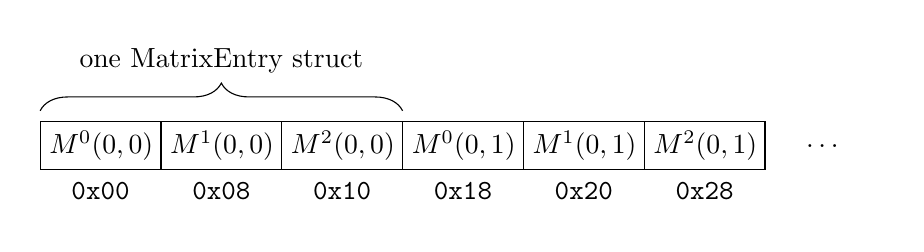
\begin{tikzpicture}[
    every node/.style={align=center, minimum height=1.5em, minimum width=1.5cm,node distance=0pt},
    background rectangle/.style={fill=black!0},show background rectangle, 
    ]
\node [cell](n1) at (0,0) {$M^0(0,0)$};
\node [cell, right = of n1] (n2) {$M^1(0,0)$};
\node [cell, right = of n2] (n3) {$M^2(0,0)$};
\node [cell, right = of n3] (n4) {$M^0(0,1)$};
\node [cell, right = of n4] (n5) {$M^1(0,1)$};
\node [cell, right = of n5] (n6) {$M^2(0,1)$};
\node [right = of n6](n7){\dots};
%\node [cell,right = of n7]{$M^2(n,m)$};

\node [below = of n1]{\texttt{0x00}};
\node [below = of n2]{\texttt{0x08}};
\node [below = of n3]{\texttt{0x10}};
\node [below = of n4]{\texttt{0x18}};
\node [below = of n5]{\texttt{0x20}};
\node [below = of n6]{\texttt{0x28}};

\draw[
   decorate,
  decoration={brace,amplitude=10pt}
]
  ([yshift=4pt]n1.north west) -- 
  node [black,yshift=18pt] {one MatrixEntry struct}
  ([yshift=4pt]n3.north east) ;

\end{tikzpicture}
\caption{Array-of-Structs data structure used to store the three matrices in memory. Each \texttt{MatrixEntry} stores the entries of a single coordinate for all three matrices. The structs are stored contiguously, as the figure depicts, in row-major order.}
\label{fig:aos}
\end{figure}

\newpage

\paragraph{Other Storage Attempts}
\label{par:otherattempts}
Since each iteration in the dynamic programming step accesses the top, left and upper-diagonal elements of the matrices, a wavefront-like storage of the matrix (see Figure~\ref{fig:wavefront}) entries yields the lowest amount of expected cache misses. Finding an easy to compute closed formula that maps the index position $(i,j)$ depicting row and column of a matrix to wavefront-coordinates turned out to be a challenge. The index of the diagonal is $i+j$, the sum of row index and column index. Finding the number of elements in the diagonal and especially the correct position within the diagonal proved more difficult though.
Since we did not find an easy formula for the mapping, we tried to store the precomputed mappings of index positions into an extra matrix. This still slowed down the program as computing the mapped indices required more arithmetic operations than we needed for the TKF algorithm.
Figure~\ref{fig:offset} shows the main problem that has to be solved in order to make wavefront indexing effective: Given an wavefront index $k$, how do we obtain the indices for the upper, upper-left-diagonal and left element of the matrix? While the needed offsets stay the same within a diagonal, they change between different diagonals in the matrix.

\begin{figure}

\begin{minipage}{0.5\textwidth}
\centering
\begin{tabular}{|c|c|c|c|c|}
\hline 
0 & 1 & 2 & 3 & 4 \\ 
\hline 
5 & 6 & 7 & 8 & 9 \\ 
\hline 
10 & 11 & 12 & 13 & 14 \\ 
\hline 
15 & 16 & 17 & 18 & 19 \\ 
\hline
\end{tabular}
\caption{Row-major indexing}
\label{fig:rowmajor}
\end{minipage}
\begin{minipage}{0.5\textwidth}
\centering
\begin{tabular}{|c|c|c|c|c|}
\hline 
0 & 1 & 3 & 6 & 10 \\ 
\hline 
2 & 4 & 7 & 11 & 14 \\ 
\hline 
5 & 8 & 12 & 15 & 17 \\ 
\hline 
9 & 13 & 16 & 18 & 19 \\ 
\hline 
\end{tabular}
\caption{Wavefront indexing}
\label{fig:wavefront}
\end{minipage}
\end{figure}

\begin{figure}
\centering
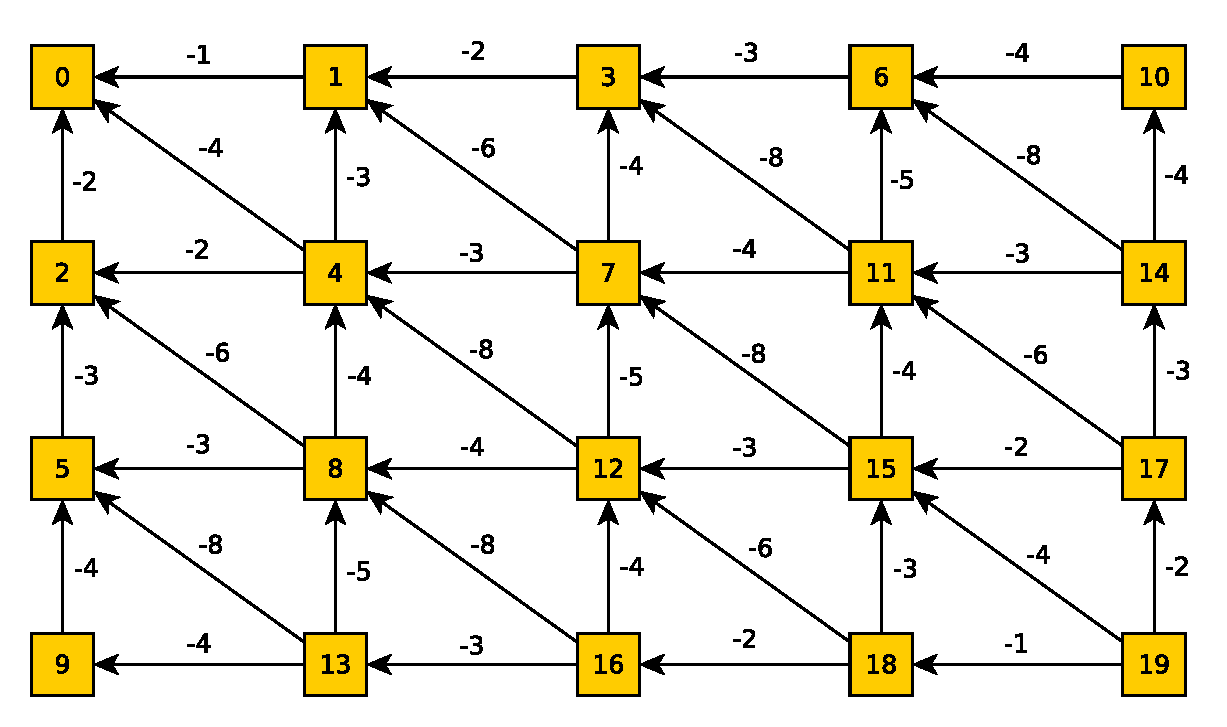
\includegraphics[scale=0.5]{images/unnamed0.pdf}
\caption{Offsets in wavefront indexing}
\label{fig:offset}
\end{figure}

%\section{Further Performance Tuning}
%- crlibm library
%- fixed-size array, no memset
%- store sequences as array of integers, used as a fast way to index precomputed logarithm values
%- fill matrices simultaneously (in the same loop)

\section{Vectorization Attempts}
\label{sec:vector}
Over the course of the practical we conducted partial vectorization of two of our implementations: the basic Log-space implementation (Section~\ref{sec:log}) and the improved Log-space implementation, using a more cache efficient data structure to store the matrices (Section~\ref{sec:caching}).

In both cases we directed our focus primarily to vectorization of the part of the code that  initializes the three matrices. Our analysis using \texttt{Valgrind callgrind} has revealed this portion to be the part in which $75-80\%$ of the runtime of the program is spent. Additionally, as the initialization calculations of each element in the three matrices are independent of each other, it presented itself as \textit{embarrassingly parallel}.

There are several steps that we took to vectorize code in both instances. First, for vector intrinsics to function correctly, it had to be assured that the respective \texttt{load} and \texttt{store} operations only interact with correctly aligned memory addresses. Secondly, we neede to find an appropriate strategy to determine how to iterate through the matrices, and how to handle matrix dimensions that are not divisible by the width of the type of vector intrinsic used. Lastly we needed to store all calculation parameters in the appropriate vector types and we had to supplant all basic operations of the calculation by their respective vector intrinsics counterparts.

\subsection{Log-space implementation}
For the vectorization of the basic Log-space implementation we ensured correct alignment of memory using the \texttt{\_\_attribute\_\_(aligned(\textit{size}))} keywords for stack allocation, and the \texttt{posix\_memalign} function for heap allocation.

As a consequence, we had to change the iteration through the matrices to start at entry $0$ of each row, as starting iteration at position $1$ would result in memory access of the vector functions of not correctly aligned memory. Furthermore, as we stored the rows of the matrices contiguously in memory, we had to increase the size of the rows so as to ensure the correct alignment of every first entry of each row.

The strategy we chose to deal with row dimensions that are not divisible by the width of the vector operations was straight forward: compute as much of the row through vector intrinsics as possible, then compute the rest sequentially. 

\subsection{Version using Array of Structs data structure}
While the strategy to deal with unfit row dimensions remained the same in the improved version of our program, we had to make several other major adjustments to be able to use vectorization in conjunction with the more cache-efficient data structure.

As Figure~\ref{fig:aos} shows, using the Array-of-Structs way allocating the matrices results in non-contiguous storing of the entries of the rows. Consequently the standard way of loading and storing values using the vector data types cannot be used here. As a workaround we implemented load and store operations specifically tailored to our data structure using vector functions that load and store single double values. An upside of this approach was that correct data alignment was no longer required. However we believe that this approach also carries significant performance overhead over the classically used operations.

\subsection{Thoughts on wavefront vectorization}
As the dynamic programming step of the TKF91 algorithm has data dependencies to the cells left of, above and diagonally left above of the cell to be computed, parallelization would require a \textit{wavefront} approach.

In wavefront parallelism, matrix entries are not computed by row or by column, but rather by computing the entries of each \textit{counter-diagonal}. Crucially, the counter-diagonals have to be computed sequentially and in-order when dependencies exist between a counter-diagonal and its previous neighbor. In this case, the current counter-diagonal is called the wavefront, giving this paradigm its name.

As the log-space transformed version of TKF91 reduces the operations that would require such a wavefront approach for parallelization to finding the greatest of two to three values, the relative amount of time spent doing so represents a negligible part of the overall algorithm. Nevertheless, we invested some time attempting a wavefront-vectorized version of the program.

Primarily, we attempted to find a suitable way of storing and accessing the cells of the matrices, such that data would be contiguous in the just described wavefront pattern rather than using row-major order. However we concluded that merely accessing a cell, using the usual row-, and column coordinates, would require significant computation by itself. Most importantly, it would require significantly more operations than the actual computations done for each matrix entry.

Compounding to this realization was, that our preliminary benchmarks had shown absolutely no increase in performance using vectorization of either major implementation. Consequently we abandoned wavefront parallelization for this algorithm.

\section{Benchmarking Results}

We conducted all measurements on a desktop machine with $16$ GB RAM and
a Intel\texttrademark~i7-2600 CPU with $4$ physical cores and hyper-threading.

\subsection{Different Logarithm Libraries}
\label{sec:crlibm}

Additionally to using the \texttt{log} function from the standard C++ header \texttt{<math.h>}, we also used the \texttt{crlibm} library by Daramy et al.~\cite{Daramy04}. It includes versions of the natural logarithm computation, which allows the type of rounding to be explicitly specified.

In order to check the correctness of our resulting alignments, we computed the edit distance between the alignments we obtained by using different logarithm implementations. We assigned a cost of $1$ to insertions, deletions and substitutions of single letters. We picked all pairs of sequences from the \\ \texttt{BDNF\_unaligned\_sequences.fas} data set from \url{http://www.uni-oldenburg.de/fileadmin/user_upload/biologie/ag/systematik/download/Programs/benchMark_data.tar.gz}.

For the remaining parameters, we used $\lambda=1, \mu=2, \pi = (0.27, 0.24, 0.26,0.23)$ and $\tau = 0.1$. The edit distances were computed in relation to using the logarithm function from \texttt{Boost.Multiprecision}. 

In particular the \texttt{log\_ru} function, which explicitly rounds up, produces a notable change in alignment compared to the logarithm function from \\ \texttt{Boost.Multiprecision} as can be seen in Table~\ref{fig:dist}. The computed likelihood scores were highly similar and the differences in the alignments were minimal as can be seen in Figure~\ref{fig:alignments}. We finally decided to use the \texttt{log\_ru} function from the \texttt{crlibm} library because it had the most consent with the alignments returned by the reference implementation (\url{http://sco.h-its.org/exelixis/web/teaching/practical15/scaledCode/tkf91_scaling.tar.gz}).

\begin{table}[h!]

\centering

\begin{tabular}{|c|c|}
\hline 
Logarithm Function & Average Edit Distance \\ 
\hline 
\texttt{log} from \texttt{<math.h>} & 2.15 \\ 
\hline 
\texttt{log\_ru} from \texttt{crlibm} & 33.15 \\ 
\hline 
\end{tabular} 
\caption{Average edit distances from the alignment returned by using  \texttt{Boost.Multiprecision} of different logarithm implementations.}
\label{fig:dist}
\end{table}


\begin{figure}

\textbf{Alignment using standard C++ header \texttt{<math.h>}}
~
\\
\texttt{ACGACTAGTCA-GC-TACG-AT-CGA-CT-C-ATTCAACTGACTGACA-TCGACTTA} \\
\texttt{A-GAG-AGTAATGCATACGCATGC-ATCTGCTATT\textcolor{red}{\underline{---C}}TG-CTG-CAGTGG--T-A}
\\~\\
\textbf{Alignment using \texttt{Boost.Multiprecision}}
~
\\
\texttt{ACGACTAGTCA-GC-TACG-AT-CGA-CT-C-ATTCAACTGACTGACA-TCGACTTA} \\
\texttt{A-GAG-AGTAATGCATACGCATGC-ATCTGCTATT\textcolor{red}{\underline{---C}}TG-CTG-CAGTGG--T-A}
\\~\\
\textbf{Alignment using \texttt{log\_ru}}
~
\\
\texttt{ACGACTAGTCA-GC-TACG-AT-CGA-CT-C-ATTCAACTGACTGACA-TCGACTTA} \\
\texttt{A-GAG-AGTAATGCATACGCATGC-ATCTGCTATT\textcolor{red}{\underline{C---}}TG-CTG-CAGTGG--T-A}
\\~\\
\textbf{Alignment from reference implementation}
~
\\
\texttt{ACGACTAGTCA-GC-TACG-AT-CGA-CT-C-ATTCAACTGACTGACA-TCGACTTA} \\
\texttt{A-GAG-AGTAATGCATACGCATGC-ATCTGCTATT\textcolor{red}{\underline{C---}}TG-CTG-CAGTGG--T-A}

\caption{Difference in alignments using the input parameters $\pi=(0.25,0.25,0.25,0.25), \lambda=1, \mu = 2, \tau = 0.1$}
\label{fig:alignments}
\end{figure}

\subsection{Runtime Measurements}

The input sequences used to measure execution time were four pairs of randomly generated sequences of length $10$, $100$, $1000$ and $10000$ nucleotides. Sequences did not contain ambiguous characters. 

We measured the execution times around the kernel of the program, that is excluding any I/O required to load parameters and input sequences, or output of the algorithm. Kernel execution was performed multiple times per input and subsequently averaged. The number of runs executed was dependent on the size of the input, so as to balance accuracy and overall benchmark time (see Table~\ref{fig:runs}). 

\begin{table}
\centering

\begin{tabular}{|c|c|}
\hline 
Length of Sequence & Number of Runs \\ 
\hline 
$10$ & $10000$ \\ 
\hline 
$100$ & $1000$ \\ 
\hline 
$1000$ & $100$ \\ 
\hline 
$10000$ & $10$ \\ 
\hline 
\end{tabular}
\caption{Number of runs per sequence length}
\label{fig:runs}
\end{table}

\begin{figure}[h!]
\includegraphics[width=\textwidth]{images/benchplot.png}
    \caption{Comparison of average run times of the different implementations. \texttt{sse3} and \texttt{avx} post-fixes denote the vectorized versions of the programs, using SSE3 and AVX vector intrinsics respectively (Section~\ref{sec:vector}). \texttt{log} denotes, that a version built on the log-space transformed version of TKF91 (Section~\ref{sec:log}). Versions using the Array-of-Structs method of storing matrices (Section~\ref{sec:caching}) are denoted by the \texttt{caching}-keyword, and the \texttt{round\_up}-keyword denotes the use of the \texttt{crlibm} library logarithm function \texttt{log\_ru} (Section~\ref{sec:crlibm}).}
\label{fig:runtime}
\end{figure}

\newpage

\section{Future Directions}

\paragraph{Compensated Summation}
Since the addition of the logarithms remains our main source of numerical error, one could try to use a compensated summation algorithm like the Kahan summation algorithm~\cite{Kahan} instead of naive summation. The advantage of the Kahan summation algorithm is that it reduces the numerical error of a summation while not depending on special data types. Moreover, it does not add much computational overhead and is easy to implement.
%More approaches worth trying are summarized well at stackoverflow.com~\cite{stackoverflow}.

\paragraph{Indexing by Diagonals}
As explained at the end of Section~\ref{par:otherattempts}, we did not find an easy way to compute the wavefront indices of neighbouring matrix entries. Another possible approach to do wavefront indexing would be to use a data structure that stores each wavefront diagonal in a separate array, as depicted in Figure~\ref{fig:wavestruct}. One could then reorganize our Array-of-Structs data structure using this approach instead of the row-major indexing.

In order to access the left and upper neighbour of a \texttt{MatrixEntry}, we need to do a case distinction: For the first $\max\{n+1,m+1\}$ diagonals, depicted in green in Figure~\ref{fig:wavestruct}, it holds that the left neighbour of a \texttt{MatrixEntry} at position $i$ in the array for the $k$th wavefront diagonal is placed at position $i$ in the array for the $(k-1)$th diagonal. The upper neighbour is at position $i-1$ in the array for the $(k-1)$th diagonal.
For the remaining $\min\{n,m\}$ diagonals, the left neighbour of a \texttt{MatrixEntry} at position $i$ in the array for the $k$th wavefront diagonal is placed at position $i+1$ in the array for the $(k-1)$th diagonal. The upper neighbour is at position $i$ in the array for the $(k-1)$th diagonal.

While accessing the upper and left element becomes straight-forward this way, finding the correct way to access the upper-left diagonal element seems tricky on the first thought. But since we can go up and then left instead of going upper-left directly, the formula for the upper-left neighbour follows immediately. 

Since we already store each wavefront diagonal separately in this storage approach, we expect it to be a good solution in order to make future wavefront vectorization attempts of the TKF algorithm easier and faster. We also hope to improve data locality by using this approach instead of the row-major indexing.

\begin{figure}[h!]

\centering
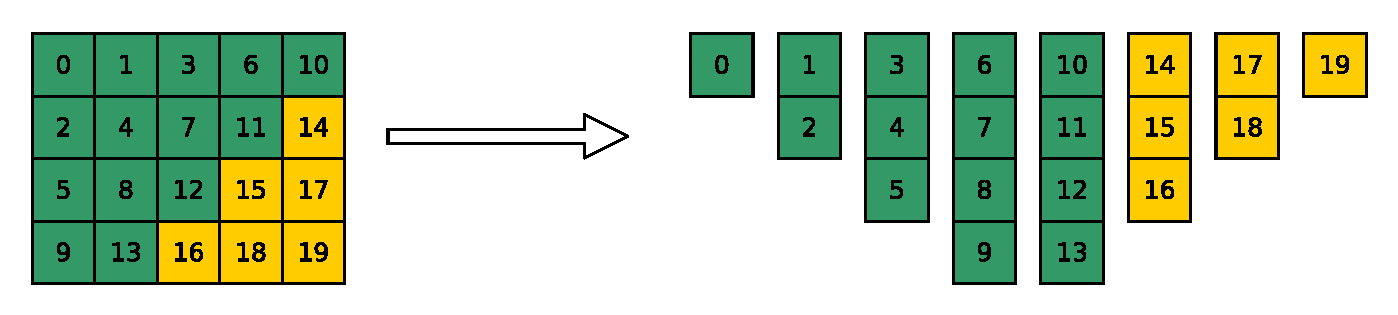
\includegraphics[scale=0.5]{images/bydiag.pdf}

\caption{Storing each wavefront diagonal in a separate array. The first $\max\{n+1,m+1\}$ diagonals are drawn in green colour.}
\label{fig:wavestruct}
\end{figure}

%This approach can also help to find a fast solution for computing neighbouring wavefront indices: If we store the prefix sums of number of elements in each wavefront diagonal, 

\bibliographystyle{plain}
\bibliography{tkf}

\begin{appendix}
\section{Formulas}

\label{sec:formulas}

In the following formulas, $1 \leq i \leq n$ and $1 \leq j \leq m$, if not specifically denoted otherwise.

\subsection{Initialization of the Matrices}
\label{sec:formulas:init}
\begin{align*}
M^0(0,0) &= -\infty \\
M^1(0,0) &= \log(\gamma_0) + \log(\zeta_1)
		= \log(1-\frac{\lambda}{\mu}) + \log (1 - \lambda * \beta) \\
M^2(0,0) &= -\infty \\
M^0(1,0) &= \log(\gamma_1) + \log(\zeta_1) + \log(\bar{p_0}) + \log(\pi_{a_1}) \\
		&= \log(1- \frac{\lambda}{\mu}) + \log(\lambda) + \log(1- \lambda *\beta) + \log(\beta) + \log(\pi_{a_1}) \\
M^0(i,0) &= M^0(i-1,0) + 2*\log(\lambda) + 2*\log(\beta) + \log(\pi_{a_i}), i \geq 2 \\
M^1(i,0) &= -\infty \\
M^2(i,0) &= -\infty \\
M^0(0,j) &= -\infty \\
M^1(0,j) &= -\infty \\
M^2(0,1) &= \log(\gamma_0) + \log(\zeta_2) + \log(\pi_{b_1}) \\
		&= \log(1- \frac{\lambda}{\mu}) + \log(1-\lambda*\beta) + \log(\lambda) + \log(\beta) + \log(\pi_{b_1}) \\
M^2(0,j) &= M^2(0, i-1) + \log(\lambda) + \log(\beta) + \log(\pi_{b_i}), j \geq 2 \\
\end{align*}

\subsection{Further Initialization}
\label{sec:formulas:further}
\begin{align*}
M^0(i,j) &= \log(\lambda) + \log(\beta) + \log(\pi_{a_i}) \\
M^1(i,j) &= \log(\lambda) - \log(\mu) + \log(\pi_{a_i}) + \log(\max\{P_{a_i \to b_j} * \bar{p_1}, \pi_{b_j} * \bar{p_1}\}) \\
	&= \log(\lambda) - \log(\mu) + \log(\pi_{a_i}) + \log(1-\lambda * \beta) + \max \begin{cases}
	\log(P_{a_i \to b_j}) - \mu*t, \\
	\log(\pi_{b_j}) + \log(1- e^{- \mu*t} - \mu * \beta)
\end{cases} \\
M^2(i,j) &= \log(\lambda) + \log(\beta) + \log(\pi_{b_j})
\end{align*}

\subsection{Dynamic Programming Step}
\begin{align*}
M^0(i,j) &= M^0(i,j) + \max\{M^0(i-1,j), M^1(i-1,j), M^2(i-1,j)\} \\
M^1(i,j) &= M^1(i,j) + \max\{M^0(i-1,j-1), M^1(i-1,j-1), M^2(i-1,j-1)\} \\
M^2(i,j) &= M^2(i,j) + \max\{M^1(i,j-1), M^2(i,j-1)\}
\end{align*}

\vspace{-1cm}
\end{appendix}

\end{document}